% The MEW nozzle in two dimensions: a short results note.
% Build: make -C paper/mew_nozzle   (figures: make -C paper/mew_nozzle figs, after the runs)
\documentclass[10pt,a4paper]{article}
\usepackage[T1]{fontenc}
\usepackage[utf8]{inputenc}
\usepackage{sourceserifpro}
\usepackage{sourcesanspro}
\renewcommand{\familydefault}{\rmdefault}
\usepackage[a4paper,margin=2.1cm,top=1.8cm,bottom=2.0cm]{geometry}
\usepackage{graphicx}
\usepackage{booktabs}
\usepackage{tabularx}
\usepackage{array}
\usepackage{microtype}
\usepackage[mode=text]{siunitx}
\usepackage{xcolor}
\usepackage{enumitem}
\usepackage{titlesec}
\usepackage[font={small,sf},labelfont={bf,sf},labelsep=period,skip=4pt]{caption}
\usepackage[colorlinks=true,linkcolor=melt,urlcolor=melt]{hyperref}

\definecolor{melt}{HTML}{2A78D6}
\definecolor{inktwo}{HTML}{4F4E4A}
\definecolor{inkthree}{HTML}{807F79}

\titleformat{\section}{\sffamily\bfseries\large}{\thesection}{0.6em}{}
\titlespacing*{\section}{0pt}{10pt}{4pt}
\titleformat{\subsection}{\sffamily\bfseries\normalsize}{\thesubsection}{0.6em}{}
\titlespacing*{\subsection}{0pt}{7pt}{2pt}
\setlength{\parskip}{3pt}
\setlength{\parindent}{0pt}
\setlist{nosep,leftmargin=1.2em,topsep=2pt}
\renewcommand{\arraystretch}{1.15}
\newcolumntype{L}{>{\raggedright\arraybackslash}X}
\newcommand{\mmcs}{\unit{\cubic\milli\metre\per\second}}

\hypersetup{pdftitle={The MEW nozzle in two dimensions},pdfauthor={Alessandro De Rosis}}

\begin{document}

{\sffamily\footnotesize\color{inkthree}M3LB \textperiodcentered{} lattice Boltzmann \textperiodcentered{} planar model\hfill 4 November 2026\par}
\vspace{6pt}
{\sffamily\bfseries\LARGE The MEW nozzle in two dimensions\par}
\vspace{3pt}
{\sffamily\large\color{inktwo}Results at the corrected feed, for the set-up of Ju, Omar, Mirihanage and Kilic\par}
\vspace{3pt}
{\small Alessandro De Rosis\par}
\vspace{8pt}

\textbf{Summary.} The set-up of \emph{Suppressing oozing during filament-based melt electrowriting}
(SSRN 7582986) was simulated as a planar slice through the nozzle: PCL at \qty{120}{\celsius} fed
through a \qty{0.4}{\milli\metre} nozzle at \qty{6.5}{\kilo\volt}, \qty{5.5}{\milli\metre} above a
collector moving at \qty{35}{\milli\metre\per\second}, at the corrected feed of
\qty{0.0208}{\cubic\milli\metre\per\second} (Table~1 prints \qty{0.255}{\cubic\milli\metre\per\second}).
Four results:
\begin{itemize}
  \item With the field off, the melt hangs from the nozzle as a drop that grows at the feed rate and
    reaches the collector after \qty{91}{\second} at the measured viscosity, \qty{820}{\pascal\second}
    (105 to \qty{110}{\second} at a nominal \qty{500}{\pascal\second}); nothing in a planar model can carry
    it away as a jet.
  \item With the field on, the result depends on how deep the model lets the melt conduct. The melt's
    estimated conductivity makes the whole drop a conductor; the field then pulls it into a column that
    reaches the collector \qty{27}{\second} before the field-off drop. Shallower conducting depths delay
    it instead, so this rests on that estimate.
  \item At \qty{35}{\milli\metre\per\second} a straight fibre carrying the whole feed is
    \qty{27.5}{\micro\metre} across; the reported \qtyrange{19}{22}{\micro\metre} fibres carry about half
    of it, the fan's \qtyrange{9.5}{13.5}{\micro\metre} fibres 12 to \qty{24}{\percent}. Neither the Taylor
    cone nor the lag angle can account for the rest.
  \item The numbers are not grid-converged, even with the melt pinned at the nozzle's edge, and nothing after
    the melt reaches the collector can be used.
\end{itemize}

\section{Model and set-up}

\begin{tabularx}{\textwidth}{@{}>{\leavevmode\sffamily\small\color{inktwo}}p{2.2cm}L@{}}
\toprule
Melt & PCL held at \qty{120}{\celsius}. Viscosity measured: 780 to \qty{850}{\pascal\second}, close to
  Newtonian from 0.4 to \qty{16}{\per\second} (the bore flow is about \qty{3}{\per\second}); runs at
  \qty{820}{\pascal\second} and at a nominal \qty{500}{\pascal\second}. Surface tension
  \qty{0.03}{\newton\per\metre} is nominal; density \qty{1080}{\kilo\gram\per\cubic\metre}. \\
Nozzle & \qty{0.4}{\milli\metre} bore, as in the paper; an assumed \qty{1.0}{\milli\metre} tip face,
  \qty{5.5}{\milli\metre} above the collector. \\
Field & \qty{6.5}{\kilo\volt}. The melt conducts down to a chosen depth below the tip (\qty{2}{\milli\metre}
  by default; 1, 3 and \qty{5}{\milli\metre} tested) and is an insulator below it, so it cannot short the gap. \\
Collector & \qty{35}{\milli\metre\per\second} (\qty{2100}{\milli\metre\per\minute}), as in every experiment. \\
Feed & \qty{0.0208}{\cubic\milli\metre\per\second}, Table~1's corrected value (Murat Kilic, 3 November),
  with and without the fan; the melt leaves the bore at \qty{0.17}{\milli\metre\per\second}. The note of
  3 November has the two earlier readings. \\
Grid & \qty{25}{\micro\metre} cells over an $8 \times 6.8$\,mm slice, \qty{14}{\micro\second} steps, and
  \qty{50}{\micro\metre} cells as a check. A free-surface lattice Boltzmann model of the melt (D2Q9, central
  moments; the air is not simulated) and Laplace's equation for the potential in the air (D2Q5); the melt
  surface feels the pull $\varepsilon_0 E^2/2$. \\
\bottomrule
\end{tabularx}

\smallskip
Matched to the experiment: the capillary numbers of the feed (2.8 at \qty{500}{\pascal\second}, 4.5 at
\qty{820}{\pascal\second}) and of the collector (583, 957), the Bond number (0.014), and the ratio of electric to capillary pressure, $\varepsilon_0 V^2/\gamma R = 62$ at
\qty{6.5}{\kilo\volt}. Not matched: inertia, which is negligible in the experiment and kept small in the
model (Reynolds number at most 0.32).

\section{Results}

\subsection{Field off: a drop that reaches the collector in one and a half to two minutes}
At \qty{500}{\pascal\second} the capillary number in the bore is 2.8. The melt hangs from the nozzle as a drop that grows at the feed
rate; its lowest point falls at about \qty{0.04}{\milli\metre\per\second} and reaches the collector after
\qty{105.0}{\second} on \qty{25}{\micro\metre} cells and \qty{110.3}{\second} on \qty{50}{\micro\metre}
cells (Fig.~\ref{fig:real}), 22 times later than the printed feed's column. The melt within
\qty{1}{\milli\metre} of the tip settles at \qty{0.69}{\milli\metre\squared}, about what the printed feed
piles there. A planar sheet carrying this feed at \qty{35}{\milli\metre\per\second} would be
\qty{1.9}{\micro\metre} thick, far below the cells, so nothing carries melt away and no jet forms. In three
dimensions a drop of the same outline needs more melt, by about its width over the bore's, four to five
times here, so a round nozzle would take longer to reach the collector: an estimate, not a run. At the
measured \qty{820}{\pascal\second} the capillary number is 4.5 and the melt comes out more like a column: on
\qty{50}{\micro\metre} cells it touches at \qty{91.3}{\second}, not \qty{110.3}{\second}.

\begin{figure}[h]
  \centering
  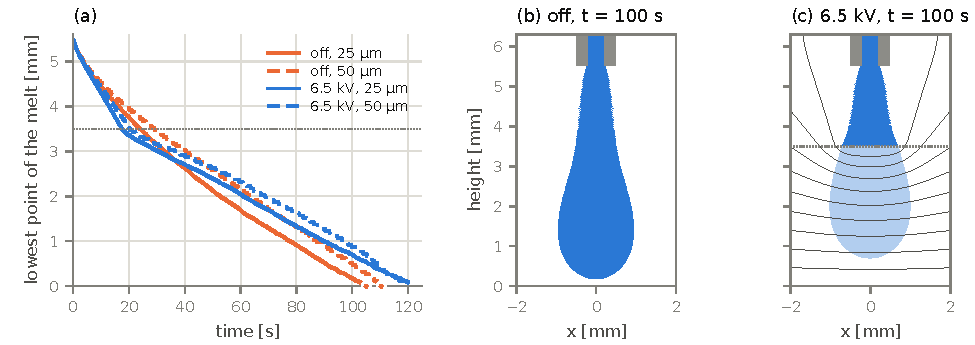
\includegraphics[width=\textwidth]{fig/fig1_real.pdf}
  \caption{The corrected feed, \qty{0.0208}{\cubic\milli\metre\per\second}, at \qty{500}{\pascal\second}. (a) Height of the lowest
    point of the melt against time with the field off (orange) and on (blue), on \qty{25}{\micro\metre}
    (solid) and \qty{50}{\micro\metre} cells (dashed). Dots mark first contact with the collector, which
    neither field-on run reaches by \qty{120}{\second}; dotted, the depth below which the melt does not
    conduct. (b, c) The drop at \qty{100}{\second} on \qty{25}{\micro\metre} cells, field off and on; in (c)
    the melt that conducts is dark and the melt below the limit light, with equipotentials every
    \qty{10}{\percent} of the voltage.}
  \label{fig:real}
\end{figure}

\subsection{Field on: later or sooner, depending on a choice in the model}\label{sec:field}
With the field on the drop first falls faster, \qty{0.40}{\milli\metre} (\qty{25}{\micro\metre} cells)
and \qty{0.45}{\milli\metre} (\qty{50}{\micro\metre}) below the field-off drop at \qty{20}{\second}. Then
it slows and widens (2.05 to \qty{2.10}{\milli\metre} at \qty{100}{\second}, against \qty{1.90}{\milli\metre})
and is still 0.09 and \qty{0.075}{\milli\metre} above the collector when the runs end at \qty{120}{\second};
extrapolated, it touches about 18 and \qty{11}{\second} after the field-off drop. The slowdown comes exactly
when the drop's lowest point leaves the zone where the model lets the melt conduct, \qty{2}{\milli\metre}
below the tip: its speed falls there from 0.090 to \qty{0.034}{\milli\metre\per\second}
(\qty{50}{\micro\metre}), while the field-off drop passes the same height unchanged at
\qty{0.05}{\milli\metre\per\second}. The model needs that limit, or the melt would short the gap, but nothing
in it fixes the depth. With the limit at 1 or \qty{3}{\milli\metre} instead (Fig.~\ref{fig:cut}a) the bend
moves with it, the runs are identical to every printed digit until the drop first passes the shallower
limit, and the drop reaches the collector 7.4, about 11 and \qty{17.0}{\second} after the field-off drop
for 1, 2 and \qty{3}{\milli\metre}.

While the whole drop conducts, its strongest pull is at its lowest point and draws it down. Once it hangs
below the limit, its conducting part ends in a flat face inside it, and the strongest pull moves to that
face's edge on the drop's sides, 7 to 56 times the typical pull on the conducting surface
(Fig.~\ref{fig:cut}b). That edge is numerical. With the limit at \qty{5}{\milli\metre}, \qty{0.5}{\milli\metre}
above the collector, the whole drop conducts until it is nearly down, as a melt whose charge relaxes in much
less than its two minutes of growth would. The field then draws it into a column that runs away toward the
collector, 2.5 to \qty{0.5}{\milli\metre} in \qty{5.5}{\second}, and it touches \qty{48}{\second}
\emph{before} the field-off drop, with 9 to \qty{14}{\kilo\volt\per\milli\metre} in the last millimetre,
well above the roughly \qty{3}{\kilo\volt\per\milli\metre} at which air breaks down. The melt's conductivity
was not measured, but its estimate, $10^{-11}$ to \qty{e-4}{\siemens\per\centi\metre}, relaxes charge in at
most about \qty{0.03}{\second}, far faster than the drop changes: the whole drop conducts, and the
\qty{5}{\milli\metre} case is the physical one. At \qty{820}{\pascal\second} it touches at
\qty{64.7}{\second}, \qty{27}{\second} before the field-off drop.

\begin{figure}[h]
  \centering
  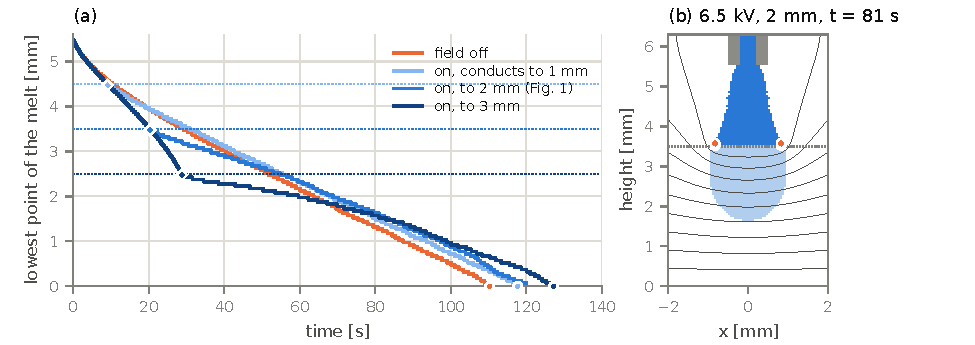
\includegraphics[width=\textwidth]{fig/fig2_cut.pdf}
  \caption{How deep the melt may conduct, on \qty{50}{\micro\metre} cells. (a) Height of the lowest point
    of the melt against time with the field off (orange) and on, the melt conducting to 1, 2, 3 or
    \qty{5}{\milli\metre} below the tip (light to dark blue; \qty{2}{\milli\metre} is the default of
    Fig.~\ref{fig:real}). Dotted, each depth; diamonds, the drop's lowest point passing it; dots, first
    contact. (b) The \qty{2}{\milli\metre} run at \qty{81}{\second}: melt that conducts (dark) and melt that
    does not (light), equipotentials every \qty{10}{\percent} of the voltage, and the four surface cells
    pulled hardest (orange), at the edge of the conducting zone.}
  \label{fig:cut}
\end{figure}

\subsection{What the fibres carry}
A straight fibre laid at \qty{35}{\milli\metre\per\second} carries its cross-section times that speed;
carrying the whole feed it would be \qty{27.5}{\micro\metre} across. The paper's
\qtyrange{19}{22}{\micro\metre} fibres (after nozzle cleaning) carry 48 to \qty{64}{\percent} of the feed,
its \qtyrange{9.5}{13.5}{\micro\metre} fibres (with the fan) 12 to \qty{24}{\percent}. A Taylor cone holds a
fixed amount once formed, 0.3 to \qty{5}{\second} of feed, against a deficit of 0.45 to
\qty{1.1}{\cubic\milli\metre} every minute. A lag angle thins the jet, but a fibre lying on the collector
moves with it, so a \qty{20.5}{\micro\metre} fibre carrying the whole feed would have to be laid at
\qty{63}{\milli\metre\per\second}, which coils it. At the same setting and speed the fan's fibres carry about a
third of the melt of those without, and no oozing is seen, which suggests the drive delivers less than its
setting with the fan on (question~1).

\subsection{How the numbers depend on the cell size}\label{sec:cells}
Nothing converges, and the nozzle is why. With no wetting the model treats the nozzle as a surface the
melt does not wet, so the melt leaves from the edge of the bore and creeps exactly two cells onto the tip
face, whatever a cell measures: the neck is 0.60, 0.50 and \qty{0.45}{\milli\metre} wide on 50, 25 and
\qty{12.5}{\micro\metre} cells, and the column follows it. At the printed feed first contact came at 5.8,
4.7 and \qty{4.0}{\second} on the three grids; at the corrected feed the field-off drop touches at 110.3 and
\qty{105.0}{\second} on 50 and \qty{25}{\micro\metre} cells, with 0.85 and \qty{0.69}{\milli\metre\squared}
of melt within \qty{1}{\milli\metre} of the tip. Pinning the melt at the nozzle's outer edge (a wetted tip)
fixes the neck at \qty{1.0}{\milli\metre} on both grids but not the rest: the finer drop then sags more
slowly and touches about \qty{19}{\second} after the coarser one (\qty{153.5}{\second}, extrapolated, against
\qty{134.5}{\second}), so a second grid effect, in the drop, partly cancels the neck's in the runs above. It is
not diagnosed. The real nozzle is not wetted, which is the case the runs use. Nothing after contact can be
used: the collector drags the drop to the side of the \qty{8}{\milli\metre} box within \qty{2}{\second}, and
the two grids then do different things.

\section{What the model leaves out}
\textbf{Three dimensions}: a planar meniscus has no conical equilibrium, the jet is far below the grid, a flat
tip concentrates the field less than a round one, and a planar drop holds less melt for its outline.
\textbf{Charge and current}: the melt is a perfect conductor down to a chosen depth and an insulator below.
\textbf{Heat}: the melt is held at \qty{120}{\celsius}; the hot end, where the fan acts, was modelled
separately. The melt is Newtonian, which the measured curve supports at the nozzle's shear rates.

\section{How far to trust it}

\begin{tabularx}{\textwidth}{@{}>{\raggedright\arraybackslash\sffamily\small}p{5.0cm}L@{}}
\toprule
Electric pull, against exact solutions &
  Its pattern is right to \qty{0.05}{\percent}, a moving surface's response to \qty{3}{\percent} once the
  surface's own stiffness is allowed for: deflections of one or two cells come out
  \qtyrange{9}{25}{\percent} short. \\
Surface tension, Laplace's law &
  Right to \qty{1.2}{\percent} for drops of 12 cells or more, \qty{3.4}{\percent} at 8 cells; the bore is 8
  cells from wall to axis. \\
Three cell sizes, 50, 25 and \qty{12.5}{\micro\metre} &
  Not converged: contact times 5 to \qty{14}{\percent} apart between 50 and \qty{25}{\micro\metre}, from the
  neck and from the drop itself (Section~\ref{sec:cells}). \\
How deep the melt conducts &
  Sets the field's effect: at \qty{500}{\pascal\second} the drop reaches the collector 7.4, about 11 and
  \qty{17.0}{\second} after the field-off drop for depths of 1, 2 and \qty{3}{\milli\metre}, and
  \qty{48}{\second} before it for \qty{5}{\milli\metre}, the case the estimated conductivity points to. \\
Mass &
  Conserved to \qty{0.3}{\percent} until contact (\qty{0.6}{\percent} at the printed feed); after contact
  off by up to \qty{3.3}{\percent}, and by up to \qty{5.4}{\percent} while a thread is drawn thin at the
  printed feed, which is not yet explained. \\
\bottomrule
\end{tabularx}

\section{Questions for the experiment}
\begin{enumerate}
  \item How much filament is drawn in over \qty{10}{\minute}, with the fan on and off? At the nominal feed it
    is \qty{5.2}{\milli\metre}; the fibres imply about half that without the fan and a fifth with it.
  \item Could the conductivity be measured, even to an order of magnitude? It would confirm that the whole
    drop conducts.
  \item Is there a surface tension for this PCL near \qty{120}{\celsius}? The model uses
    \qty{0.03}{\newton\per\metre}.
  \item With the voltage off, how long does the melt take to reach the collector? The planar model gives
    about \qty{1.5}{\minute} at \qty{820}{\pascal\second}; a round nozzle would take longer.
\end{enumerate}

\vfill
{\footnotesize\color{inkthree}\sffamily M3LB (\href{https://github.com/alexderosis/M3LB}{github.com/alexderosis/M3LB},
branch \texttt{electrowriting}), double precision: \texttt{demonstrator/mew\_nozzle -feed 0.0208} with
\texttt{-nofield}, \texttt{-mu 820}, \texttt{-lc 1}, \texttt{3} or \texttt{5}, and \texttt{-film 0.1 -wet 60} for a
wetted tip; cells \texttt{-R 8} or \texttt{-R 4 -Ucol 0.04}. Figures: \texttt{paper/mew\_nozzle/make\_figs.py}.\par}

\end{document}
